\subsection{Dữ liệu}
Được lấy từ package python fix\_yahoo\_finance. Gói này lấy thông tin từ trang Yahoo Finance và chuyển thành Panda Dataframe.
Bảng này gồm 7 cột:
\begin{itemize}
    \item Date: ngày
    \item Open: giá lúc mở phiên
    \item Close: giá lúc đóng phiên danh nghĩa
    \item High: giá cao nhất trong ngày
    \item Low: giá thấp nhất trong ngày
    \item Adj close: giá lúc đóng phiên thực tế đã tính phần lạm phát
    \item Volume: số lượng bán ra
\end{itemize}

\begin{table}[h]
	\begin{tabularx}{\textwidth}{X | X | X | X | X | X | X } 
		%\hline
		Date		& Open  & Date  & Close  & High  & Low & Adj close & Volume  		\\ \hline
		2004-11-18	& 44.43	& 44.490002	& 44.07	 & 44.380001	& 44.380001	& 5992000		\\ %\hline
	\end{tabularx}
	\label{tab:sample-data}
	\caption{}
\end{table}

\begin{figure}[!htb]
    \center{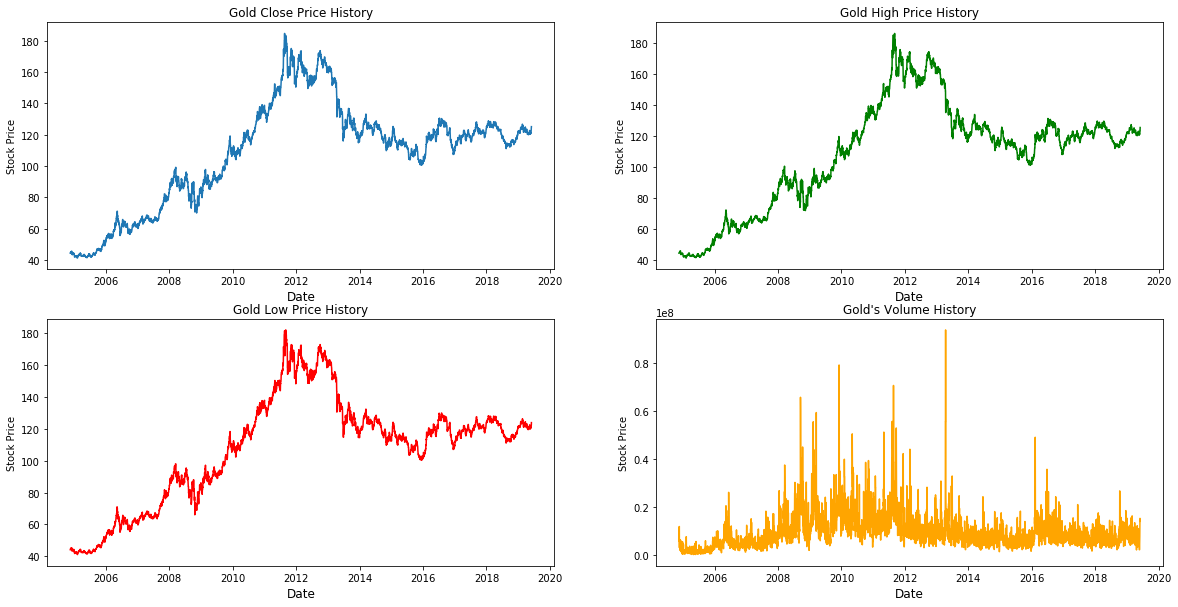
\includegraphics[width=16cm]
    {figure/data/plot.png}}
    \caption{\label{fig:gld-data} Biểu đồ dữ liệu}
\end{figure}

Dự liệu được lấy từ thị trướng chứng khoán, chính vì vậy, có những ngày nghỉ như ngày lễ, ngày thứ 7, chủ nhật sẽ không có dữ liệu.
Có vẻ như dữ liệu không có xu hướng trong năm, mùa và không bị ảnh hưởng bởi ngày lễ. Số lượng bán ra không phụ thuộc vào giá bán.

\subsection{Xử lý dữ liệu}

\textbf{Đối với mạng học sâu} \\
Chuyển thành bài toán học có giám sát
\begin{itemize}
    \item Đối với những ngày không có dữ liệu thì điền dữ liệu bằng ngày trước để có tính liên tục \\
    \item Giữ lại cột: Date, Close. Đổi tên cột Date thành ds, Close thành y. Bỏ các cột còn lại(Theo quy chuẩn) \\
    \item Chuẩn hoá dữ liệu cột y bằng MinMaxScalar với khoảng (0, 1) \\
    \item Giữ 90 ngày cuối để xác minh. Những ngaỳ còn lại để đem train \\
    \item Dữ liệu đầu vào: sẽ ra giá của 90 ngày trước ngày hiện tại \\
    Dữ liệu đầu ra là giá vàng của ngày hiện tại +  89 ngày sau ngày hiện tại. Vậy sẽ bỏ qua 90 ngày đầu của bộ dữ liệu (thiếu dữ liệu ngày trước đó). 90 ngày cuối vẫn giữ lại. Đối với những ngày không có dữ liệu thì điền vào 0 \\
\end{itemize}
\begin{table}[h]
	\begin{tabularx}{\textwidth}{X | X | X | X | X | X | X } 
		%\hline
		y\_past\_1	& y\_past\_2	 & y\_past\_3	& ...	& y\_past\_88	 & y\_past\_89	 & y\_past\_90 		\\ \hline
		0.009210	& 0.009000	& 0.005721	& ... & 0.024559	& 0.024559	& 0.021768\\ \hline
		...	& ...	& ...	& ... & ...	& ...	& ... \\ \hline
		0.512300	& 0.540010	& 0.531230	& ... & 0.550120	& 0.550300	& 0.550309\\ %\hline
	\end{tabularx}
	\label{tab:table_input}
	\caption{Dữ liệu đầu vào mẫu}
\end{table}
\begin{table}[h]
	\begin{tabularx}{\textwidth}{X | X | X | X | X | X | X } 
		%\hline
		y	& y\_future\_1 & y\_future\_2	& ...	& y\_future\_87	 & y\_future\_88	 & y\_future\_89		\\ \hline
		0.008791	& 0.010256	& 0.010396		& ... & 0.004814	& 0.004814	& 0.004326\\ \hline
		...	& ...	& ...	& ... & ...	& ...	& ... \\ \hline
		0.520001	& 0	& 0		& ... & 0	& 0	& 0\\ %\hline
\end{tabularx}
	\label{tab:table_output}
	\caption{Dữ liệu đầu ra mẫu}
\end{table}


\textbf{Đối với Prophet}
Chỉ cần đưa dữ liệu vào
\begin{itemize}
    \item Đối với những ngày không có dữ liệu thì điền dữ liệu bằng ngày trước để có tính liên tục \\
    \item Giữ lại cột: Date, Close. Đổi tên cột Date thành ds, Close thành y. Bỏ các cột còn lại(Theo quy chuẩn) \\
    \item Giữ 90 ngày cuối để xác minh. Những ngày còn lại để đem train \\
\end{itemize}
\begin{table}[h]
	\begin{tabularx}{\textwidth}{X | X } 
		%\hline
		ds	& y	  \\ \hline
		2019-03-01	& 121.879997 \\ \hline
		2019-03-02	& 121.879997 \\ \hline
		2019-03-03	& 121.823122 \\ \hline
		2019-03-04	& 121.842212 \\ \hline
		2019-03-05	& 121.851212 \\ %\hline
	\end{tabularx}
	\label{tab:data_prophet}
	\caption{Dữ liệu mẫu Prophet}
\end{table}

\subsection{Xây dựng mô hình}
\textbf{Mạng học sâu} \\
Mạng học sâu 1 gồm 5 lớp: LSTM -> Dropout -> LSTM -> Dropout -> Dense \\
\begin{minted}{python}
complex_model = Sequential()
complex_model.add(LSTM(units=100, input_shape=(X_train_vals.shape[1],
X_train_vals.shape[2]), return_sequences=True))
complex_model.add(Dropout(rate=0.2))
complex_model.add(LSTM(100, return_sequences=False))
complex_model.add(Dropout(rate=0.2))
complex_model.add(Dense(prediction_size, activation='linear'))
complex_model.compile(loss='mae', optimizer='adam')
\end{minted}
Mạng học sâu 2 lúc sau đơn giản hơn là : LSTM -> Dense \\
\begin{minted}{python}
basic_model = Sequential()
basic_model.add(LSTM(500, input_shape=(X_train_vals.shape[1],
X_train_vals.shape[2])))
basic_model.add(Dense(prediction_size))
basic_model.compile(loss='mae', optimizer='adam')
\end{minted}
Đầu vào có dạng (batch\_size, 90, 1) \\
Đầu ra có dạng (90) (dự đoán 90 ngày cùng lúc) \\
Mạng được train với loss function là \(MAE = \frac{1}{n}\sum_{i=1}^{n}|p_i - a_i|\), optimizer là Adam \\
\textbf{Prophet} \\
Prophet với tham số mặc định, sử dụng daily seasonality, weekly seasonality, daily seasonality \\
\begin{minted}{python}
m = Prophet(daily_seasonality=True,
weekly_seasonality=True, daily_seasonality=True)
\end{minted}
\subsection{Công thức để đánh giá}
Sử dụng MAE để đánh giá. \\
\[MAE = \frac{1}{n}\sum_{i=1}^{n}|p_i - a_i|\]
\begin{minipage}[t]{.27\textwidth}
	\textit{Trong đó}
\end{minipage}
\hspace*{15pt}
\begin{minipage}[t]{.65\textwidth}
	\(n\) là số ngày dự đoán \\
	\(p_i\) là kết quả dự đoán vào ngày thứ \(i\) \\
	\(a_i\) là kết quả thực tế vào ngày thứ \(i\) \\
\end{minipage} \\[5mm]


\begin{figure}[!htb]
	\center{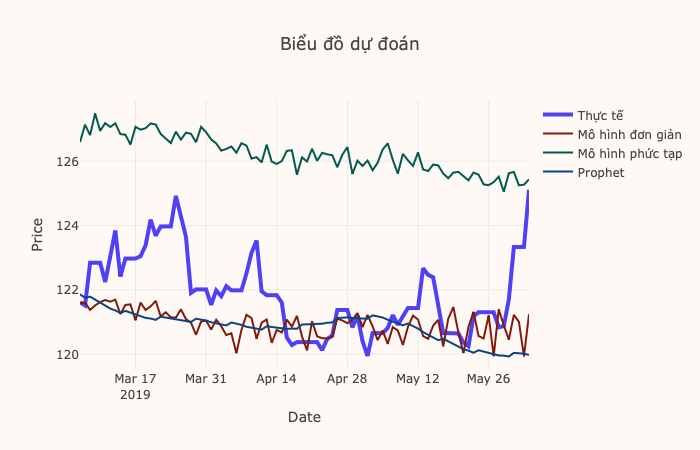
\includegraphics[width=16cm]
	{figure/result.png}}
	\caption{\label{fig:predic-res} Biểu đồ kết quả}
\end{figure}


\begin{table}[h]
	\begin{tabularx}{\textwidth}{X | X }
		%\hline
		Mô hình	& MAE	  \\ \hline
		Mạng học sâu 1	& 4.3483 \\ \hline
		Mạng học sâu 2	& 1.1131 \\ \hline
		Prophet	& 1.2269 \\
	\end{tabularx}
	\label{tab:result}
	\caption{Kết quả}
\end{table}
Đánh ngạc nhiên là mạng có cấu trúc đơn giản hơn lại đưa ra đự đoán chính xác hơn. Và prophet không tinh chỉnh nhiều tham số gì lại đưa ra kết quả chính xác hơn mạng phức tạp.
